\documentclass[dvipsnames]{beamer}
\usepackage[T1]{fontenc}
\usepackage{geometry}
\usepackage[utf8]{inputenc}
\usepackage{colortbl}
\usepackage[english]{babel}
\usepackage{pgf}
\usepackage{graphicx,epsfig, subfigure}
\usepackage{hyperref}
\usepackage{multirow}
\usepackage{minted}
\definecolor{lightgray}{rgb}{.3,.3,.3}
\usepackage{niceslides}

\title{Proofs as Programs}
\subtitle{Exercises in Type Level Programming}

% Authors
\author{
  Joachim Tilsted Kristensen
}

% Affiliations
\institute{
  Univertity of Oslo
}

\date{Kosice, 16 Nov. 2023}

\begin{document}
\frame{\titlepage \vspace{-0.5cm}}

\begin{frame}{}
  \begin{center}
    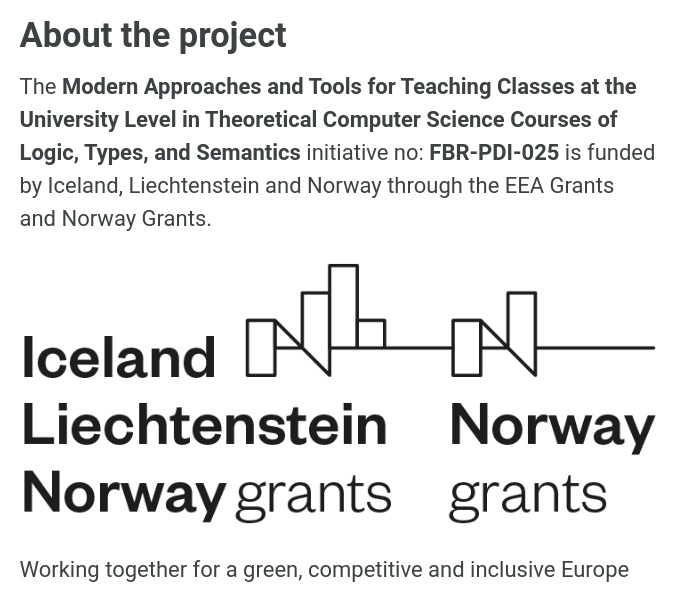
\includegraphics[width=0.8\textwidth]{logo}
  \end{center}
\end{frame}

\begin{frame}{}
  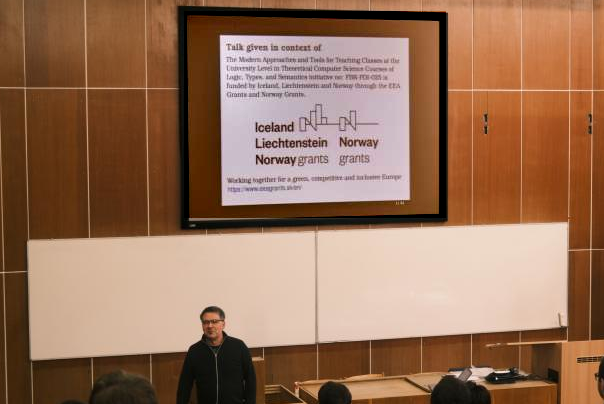
\includegraphics[width=\textwidth]{michael2}
\end{frame}

\begin{frame}{}
  \begin{center}
  \begin{block}{Agenda}
    \begin{itemize}
    \item Propositions as types, proofs as programs.
    \item Exercises.
    \item What are dependent types.
    \item How can we simulate dependent types in Haskell.
    \item Exercises.
    \item Discussion.
    \end{itemize}
  \end{block}
  \end{center}
\end{frame}

\begin{frame}{The Curry-Howard-Lambek Correspondence}
  \begin{block}{From Wikipedia}
    \begin{itemize}
    \item Curry 1934 : Types look like axiom schemes for intuitionistic logic.
    \item Curry 1958 : Hilbert style deduction systems coincide with the typed fragment of combinatory logic.
    \item Howard 1969 : Natural deduction can be directly interpreted in a typed lambda calculus.
    \item Lambek 2005 : Lambda calculi are structurally equivalent to Cartesian closed categories.
    \end{itemize}
  \end{block}
\end{frame}

\begin{frame}{Propositions as types, Proofs as Programs (Exercises)}
  \begin{center}
    \url{https://github.com/jtkristensen/exercises-in-type-level-programming/tree/main/tuke-2023/ProofsAsPrograms}
  \end{center}
\end{frame}

\frame{
  \frametitle{Lambda Cube ($\lambda_\rightarrow$)}
  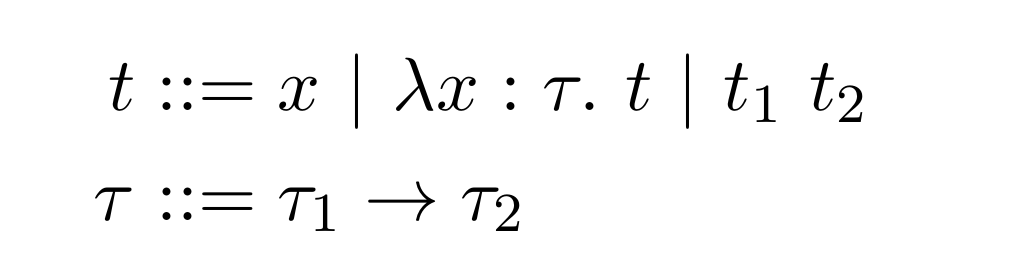
\includegraphics[width=0.5\textwidth]{./illustrations/lambda_calculus/basic_syntax}\\ \\

  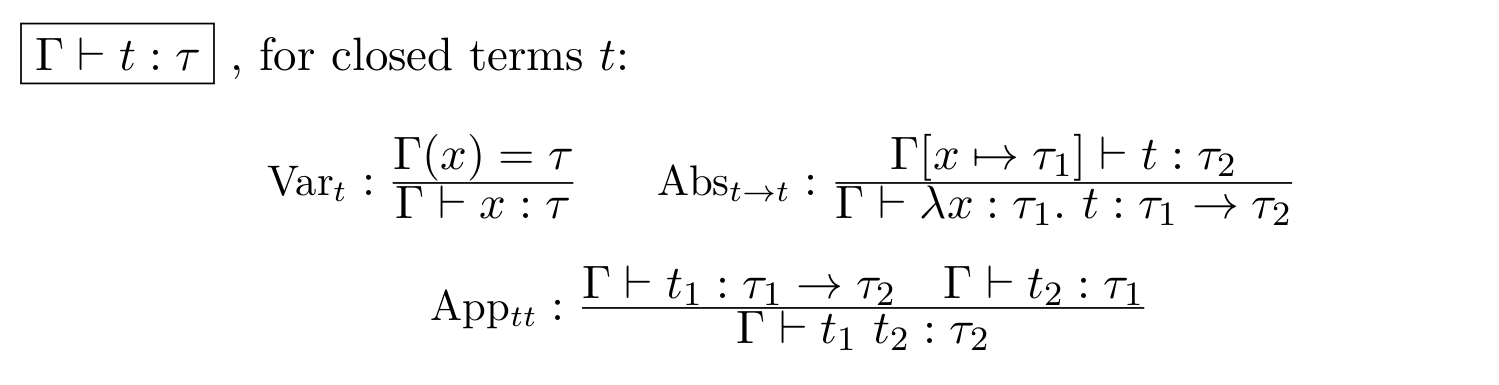
\includegraphics[width=\textwidth]{./illustrations/lambda_calculus/basic_typing}
}

\frame{
  \frametitle{Lambda Cube ($\lambda_2$)}
  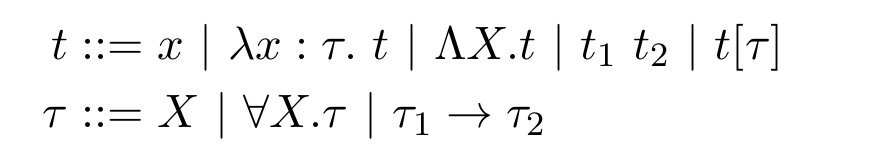
\includegraphics[width=0.5\textwidth]{./illustrations/lambda_calculus/polymorphic_syntax}\\
  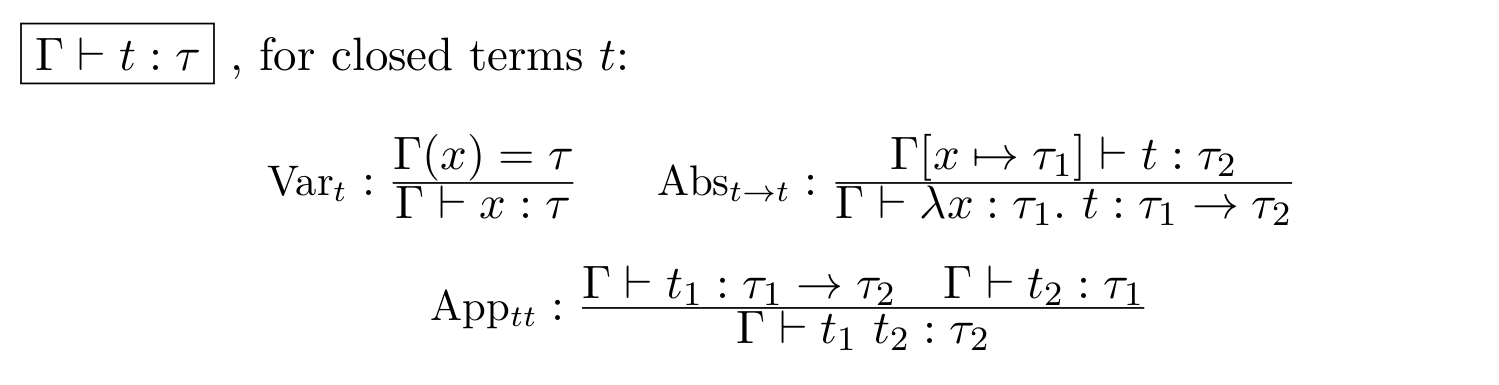
\includegraphics[width=\textwidth]{./illustrations/lambda_calculus/basic_typing}\\
  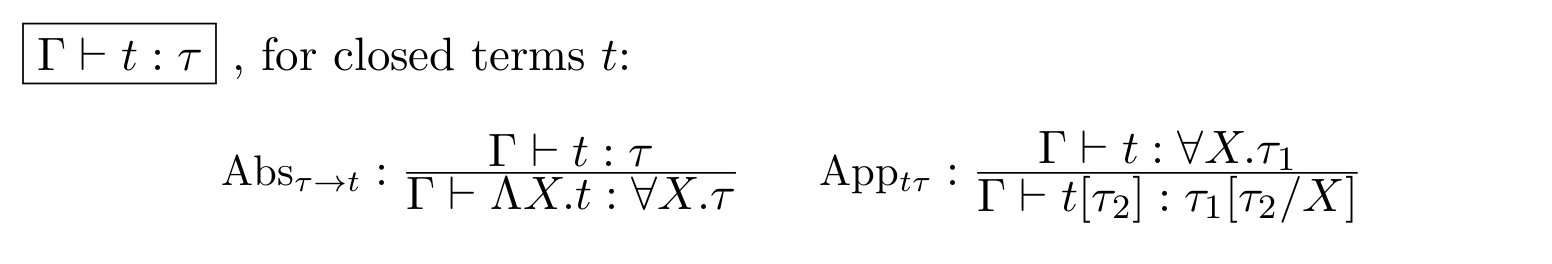
\includegraphics[width=\textwidth]{./illustrations/lambda_calculus/polymorphic_typing}
}

\frame{
  \frametitle{Lambda Cube ($\lambda_\omega$)}
  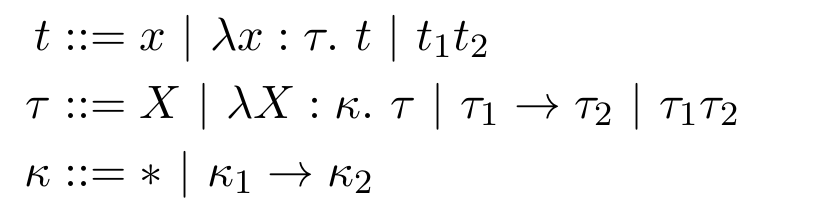
\includegraphics[width=0.5\textwidth]{./illustrations/lambda_calculus/type_level_syntax}\\
  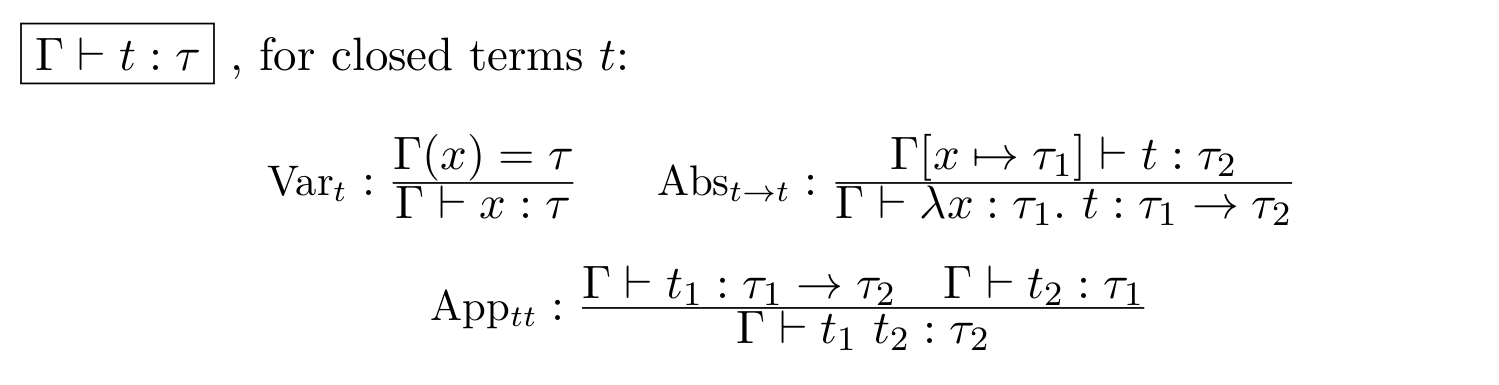
\includegraphics[width=\textwidth]{./illustrations/lambda_calculus/basic_typing}\\

  repeat Var$_t$, Abs$_{t\rightarrow{t}}$ and App$_{tt}$ to get Var$_\tau$, Abs$_{\tau\rightarrow\tau}$ and App$_{\tau\tau}$.
}

\frame{
  \frametitle{Lambda Cube ($\lambda_\Pi$)}
  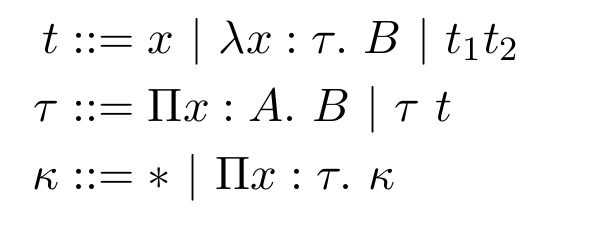
\includegraphics[width=0.5\textwidth]{./illustrations/lambda_calculus/dependent_syntax}\\
  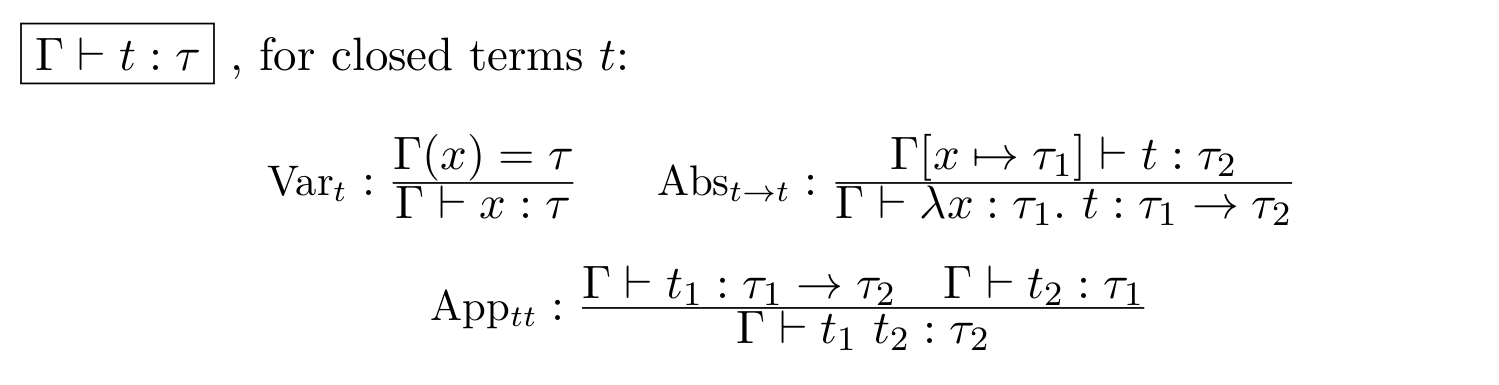
\includegraphics[width=0.9\textwidth]{./illustrations/lambda_calculus/basic_typing}\\
  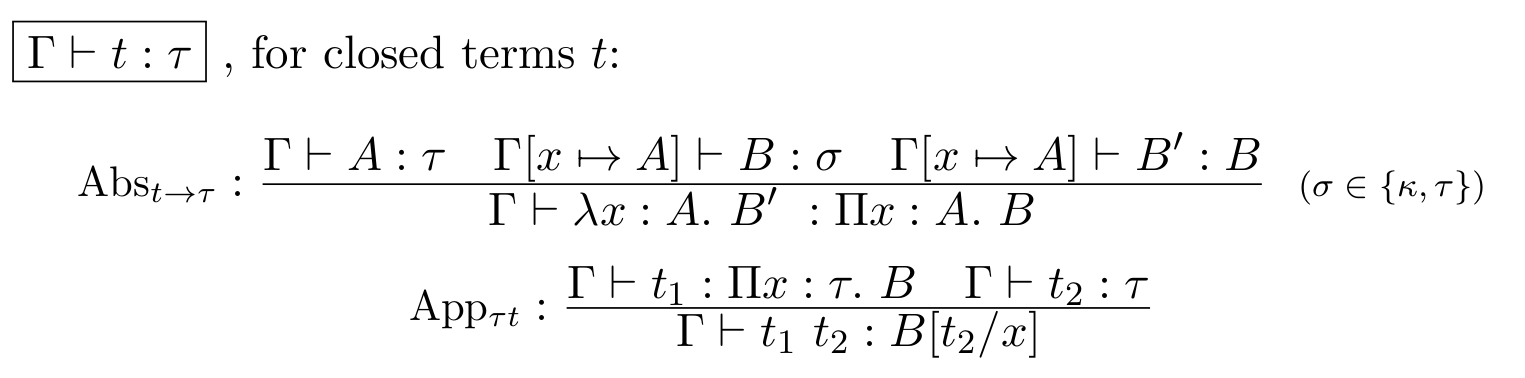
\includegraphics[width=0.9\textwidth]{./illustrations/lambda_calculus/dependent_typing}
}

\begin{frame}{Simulating Dependent types in Haskell (Exercises)}
  \begin{center}
\url{https://github.com/jtkristensen/exercises-in-type-level-programming/tree/main/tuke-2023/NatProperties}
  \end{center}
\end{frame}

\frame{
  \begin{center}
    Discussion
  \end{center}
}

\end{document}

%%% Local Variables:
%%% mode: latex
%%% TeX-master: t
%%% End:
